\pdfcompresslevel9
\pdfdecimaldigits2
\pdfminorversion4

\documentclass[10pt,a4paper]{book}
\usepackage[bottom=2.5cm,top=3.5cm]{geometry}
%\usepackage{ngerman}
\usepackage[utf8]{inputenc}
\usepackage[T1]{fontenc}
\usepackage{graphicx}
\usepackage{colortbl}
\usepackage{ae}
\usepackage{amssymb}
\usepackage{amsmath}
\usepackage{amsthm}
\usepackage{multirow}
\usepackage{rotating}
\usepackage[margin=10pt,font=small,labelfont=bf]{caption}
\usepackage{listings}
\usepackage{microtype}

%\linespread{1.25}
\setlength{\parindent}{0pt}

\usepackage{fancyhdr}
\usepackage[
  	pdfstartview=FitH,   
  	pdffitwindow=true,
	pdftitle = "Models of Computation WiSe1011 UdS", % Sets the document information Title field
    pdfauthor = "Adrian Neumann", %Sets the document information Author field
  	colorlinks,
  	linkcolor=black,
  	anchorcolor=black,
  	citecolor=black,
  	urlcolor=black
]{hyperref}

\pagestyle{fancy}
\cfoot{\thepage}

\newsavebox{\footerlicence}
\sbox{\footerlicence}{
\includegraphics{./images/by-nc-sa}}

\rfoot{\usebox{\footerlicence}}
\fancyhead{}
\lfoot{Found a mistake? Write an e-mail!}

\definecolor{gruen}{rgb}{0.5,1,0.5}
\definecolor{rot}{rgb}{1,0.5,0.5}


\renewcommand{\footrulewidth}{0.4pt}
\renewcommand{\headrulewidth}{0pt}
\newcommand{\B}[0]{\mathbb{B}}
\newcommand{\N}[0]{\mathbb{N}}
\newcommand{\Z}[0]{\mathbb{Z}}
\newcommand{\Q}[0]{\mathbb{Q}}
\newcommand{\R}[0]{\mathbb{R}}
\newcommand{\C}[0]{\mathbb{C}}
\newcommand{\E}[0]{\mathbb{E}}
\newcommand{\im}[0]{\mathit{i}}
\newcommand{\kthings}[2]{{#1}_1,\ldots,{#1}_{#2}}
\newcommand{\nthings}[1]{\kthings{#1}{n}}
\newcommand{\norm}[1]{|\!|#1|\!|}
\newcommand{\rank}{\mbox{rank }}
\newcommand{\skal}[1]{\left\langle {#1} \right\langle}
\newcommand{\ok}{{\large \checkmark}}
\newcommand{\no}{{\large $\mathbb{\times}$}}
\newcommand{\nz}{\text{nz}}
\newcommand{\rup}[1]{\left\lceil #1 \right\rceil}
\renewcommand{\bar}{\overline}
\renewcommand{\arraystretch}{1.5}
\newcommand{\argmin}[1]{\underset{#1}{\operatorname{argmin}}}
\newcommand{\var}{\operatorname{var}}
\newcommand{\Vol}{\operatorname{Vol}}



\newcommand{\trans}[1]{{#1}^\text{\upshape \sffamily T}}
\newtheoremstyle{leplain} %name
    {2em} %above
    {2em} %below
    {} %body font
    {} %indent
    {\bfseries} %head font
    {:} %punctuation after head
    {0.5em} %space after head
    {} %head spec
\title{Models of Computation}
\author{Adrian Neumann \\ {\small \texttt{adrian\_neumann@gmx.de}}}


\date{}

\begin{document}
\frontmatter
\lstdefinelanguage{pseudocode}{
    morekeywords = {repeat, until, if, else, wait, send, receive, unless, while, for, return, break},
    sensitive = false,
    morecomment=[l]{//},
    morecomment=[s]{/*}{*/},
}
\lstset{language=pseudocode, basicstyle=\sffamily\small, commentstyle=\slshape\sffamily, keywordstyle=\upshape\bfseries, breaklines=true, mathescape=true, tabsize=2}


\theoremstyle{definition}
\newtheorem{Def}{Definition}[section]

\theoremstyle{leplain}
\newtheorem{ex}{Example}[section]
\newtheorem{pr}{Proof}[section]
\newtheorem{cor}{Corollary}[section]
\newtheorem{lem}{Lemma}[section]

\theoremstyle{theorem}
\newtheorem{thm}{Theorem}[section]



\maketitle
\thispagestyle{fancy}

\section*{Disclaimer}

Most likely this script is riddled with errors so take everything with an appropriate dose of salt. Send the author emails or patches if you find errors or have some clarifications. 

These notes are released under a Creative Commons Attribution--Noncommercial--Share-Alike licence. So you can do pretty much everything with them as long as you mention the original authors, don't sell your work and distribute it under an equivalent licence. Read the licence agreement for details. Although the licence does not request it the author would be happy if you noticed him should you decide to use this.

\section*{Thanks}
The following persons have contributed:

\begin{center}
\begin{tabular}{l|c}
Name & Corrections\\\hline
Aram Harutyunan & 11
Radu Curticapean & 20
\end{tabular}
\end{center}
\newpage

\mainmatter

\chapter{Distributed Computing}

\section{Introduction}

Many autonomous entities with their own hardware (memory, CPU) in a system that connects them through a network over which they can send messages to each other. The natural way to represent that is a graph. There are many models to describe different aspects of the system. They have to deal with the following issues:

\begin{enumerate}
\item Communication. Usually communication is very expensive, its cost dominates all other costs. Hence it is typically assumed that communication is the only cost that occurs.
\item Fault Tolerance. In large computer networks it's common that a few nodes fail during the computation. Robustness against this is desirable. Results should be reasonable even if single entities fail.
\item Locality. Networks change over time, communicating these changes to all nodes would be too costly. It's better to design algorithms that only rely on local information.
\item Synchronization. Individual entities can have different hardware and solve problems at different speeds. It's good if algorithms don't have to assume synchronous computation.
\item Symmetry breaking. Nodes have to be made distinguishable.
\end{enumerate}

\section{Vertex Coloring}

Given an undirected graph $G=(V,E)$ we want to find a colouring, i.e. an assignment of colours $c_v$ to the vertices $v\in V$, such that no two adjacent vertices have the same colour.

This is useful for symmetry breaking. For example cellphones that communicate with the same cell have to choose different frequencies.

We will assume that initially all nodes are equipped with a unique ID$\in [1,n]$. Typically each ID uses $O(\log n)$ bits. Obviously the IDs are a valid colouring. We want to try to use fewer colours, if possible the minimal number.

\begin{Def}[Chromatic Number] The chromatic number $\chi(X)$ of a graph is the minimal number of colours needed in any valid colouring of G.
\end{Def}

Computing the chromatic number is NP-complete. Hence we want to try to find some approximate solution.

A simple, sequential algorithm assigns colours greedily:

\begin{lstlisting}
Greedy(graph G)
while $\exists$ uncoloured vertex v
	colour v with min ([1,n] - colours(neighb(v)))
\end{lstlisting}

\begin{thm} The greedy algorithm stops after $n$ steps and produces a valid colouring and uses at most $\Delta(G)+1$ colours\footnote{$\Delta(G)$ is the maximal degree of the graph}.
\end{thm}

\begin{pr} It is clear that the algorithm stops in $n$ steps, since in each iteration the number of vertices decreases by one. 

Correctness is given by an inductive argument. During the execution the coloured subgraph is always valid, since we assign colours that don't occur in the neighbourhood.

Finally $\Delta(G)+1$ is an upper bound for the number of colours since there is always a free colour in the set $[1,\Delta(G)+1]$ 
\end{pr}

We want to construct a distributed algorithm that uses the same ideas to reduce the number of colours.

\begin{lstlisting}
First-Free(coloured G, vertex v)
	give v the smallest available colour
\end{lstlisting}

This algorithm can produce error if two adjacent vertices choose the colour at the same time under certain circumstances.

\begin{figure}
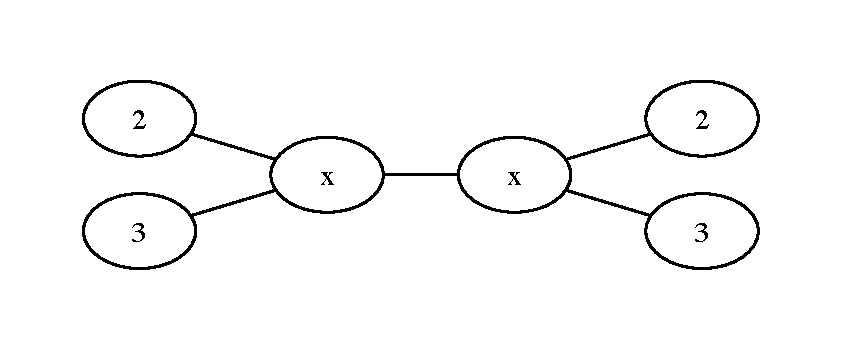
\includegraphics[width=0.5\linewidth]{./images/graph1}
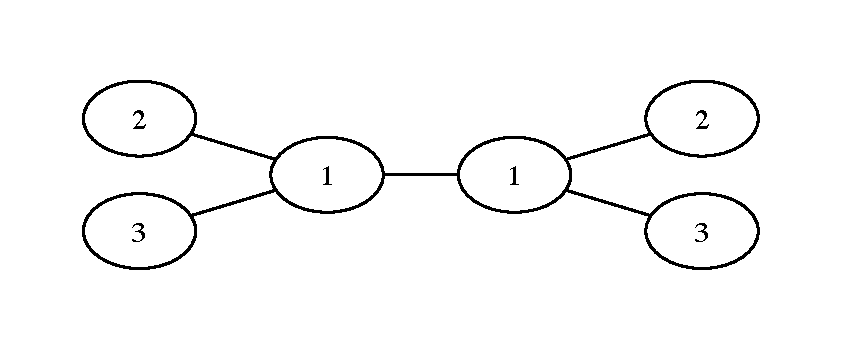
\includegraphics[width=0.5\linewidth]{./images/graph11}
\caption{If the nodes labelled with x have high IDs and choose simultaniously they produce an invalid colouring.}
%n1 2
%n2 x
%n3 3
%n4 10
%n5 2
%n6 3
%n1 -- n2
%n2 -- n3
%n2 -- n4
%n4 -- n5
%n4 -- n6
%
%n1 and n2 choose colours simultaniously, both get 1.
\end{figure}

It depends on the model how we can deal with this. Either we have the means for synchronisation, or we don't.

\begin{Def}[Synchronous Distributed Algorithm] During one unit of time an entity in a SDA can execute (in any order) the following things
\begin{itemize}
\item Perform local computations
\item Send messages
\item Receive messages
\end{itemize}

As long as they are of "reasonable" complexity
\end{Def}

In this model we can change the algorithm like this:

\begin{lstlisting}
Reduce
	send own ID to all neighbours
	receive IDs from all neighbours
	while $\exists$ uncolored vertex in the neighbourhood that has larger ID
		send "undecided" to all neighbours
		receive messages from neighbours
	colour thyself with First-Free
	send the colour to neighbours
\end{lstlisting}

\begin{thm} Reduce is correct, i.e. it produces a valid colouring after at most $n$ rounds. The number of colours used is upper bounded by $\Delta(G)+1$. 
\end{thm}

\begin{pr}
\end{pr}
\subsection{Colouring Trees}

In order to finde a faster algorithm we first look at a special case, trees. A tree is an acyclic connected graph. All trees are bipartite, and hence have chromatic number 2.

\begin{thm} $T$ is a tree implies $\chi(T)=2$ \end{thm}

\begin{pr} Let $v$ be a distinguished vertex, the root, in the tree. Colour $v$ red.  Colour every other vertex according to the distance from the root. If the distance is odd colour it blue, else red. Since there are no cycles in the graph, the coloring is valid.
\end{pr}

If we assume that the root knows that it's special we can construct the algorithm in figure \ref{alg:slow_tree_colour}

\begin{figure}[hbt]
\begin{lstlisting}
root: colour with red; send to all children
all except root: 
	wait for message
	if parent red
		colour blue
	else
		color red
	send colour to all children
\end{lstlisting}
\caption{Slow Tree Coloring}
\label{alg:slow_tree_colour}
\end{figure}


This algorithm isn't faster than the previous one, for degenerate trees. We also need to find a way to decide which node is the root. The latter problem is deferred to a later lecture.

Note that this algorithm doesn't need to operate in a synchronous environment. Every node waits for an event before it starts its computation. Event-driven algorithms can be implemented in asynchronous settings

\begin{Def}[Asynchronous DA] A asynchronous distributed algorithm has no access to a global clock and works event-driven.

Any sent message will arrive in finite time.
\end{Def}

There are different ways to assess the complexity of asynchronous algorithms (there are not bounds on the time a message takes). Typically we are interested in 

\begin{itemize}
\item Message Complexity: The number of messages sent
\item Time Complexity: Under the assumption that each message has delay 1, the time complexity is the length of the longest chain of interdependent messages.
\end{itemize}

\begin{thm} The asynchronous time complexity of algorithm \ref{alg:slow_tree_colour} is $\leq height(T)$ \end{thm}
\begin{pr} In the first round the root sends its colour to all neighbours. This costs one time unit. Argument follows from induction on the height\end{pr}

We now try to improve the algorithm to get a better runtime than $O(n)$. In fact we'll give an algorithm that is bounded by $O(\log^*n)$. We assume that all vertices know that the graph is a tree, a root is known and each node knows it's parent. How we find that information is again deferred to later

\begin{figure}[hbt]
\begin{lstlisting}
Let $c_v$ be ID(v)
repeat 
	send $c_v$ to all childrens
	if $v$ is the root then
		I=0
	else 
		let $c_p$ be the parent's colour
		I = smallest i s.t. bin$_i$($c_v$), bin$_i$($c_p$) differ
		$c_v$ = <bin(I),bin$_I$($c_v$)> //use $1+\log |c_v|$ bits  
		                                //even if I small
until |bin($c_v$)| does not change
\end{lstlisting}
\caption{6-colour}
\label{alg:6-colour}
\end{figure}

\begin{lem} Algorithm \ref{alg:6-colour} produces a valid colouring \end{lem}

\begin{pr} Since all IDs are different the colouring is valid in the first step. Now consider some iteration during the execution of the algorithm

Let $u$ be the parent of $w$. If $u$ finds $I_u$ and $w$ finds $I_w$ then the new colours are $c_u=<bin(I_u), bin_{I_u}(c_u)>, c_w<bin(I_w),b_{I_w}(c_w)>$. There are two cases

\begin{itemize}
\item $I_u\neq I_w$. Then the first part of the new colours differ. \ok
\item $I_u=I_w=I$. Then we have $b_I(c_u)\neq b_I(c_w)$, by the choice of $I$ \ok
\end{itemize}

So the colouring stays valid after each round.
\end{pr}

\begin{lem} Let $K_i$ be the number of bits in the representations of the colours in round $i$.

\begin{align*}
K_0 &= \left\lceil \log n\right\rceil\\
K_{i+1} &= 1+\left\lceil K_i\right\rceil
\end{align*}

\end{lem}

\begin{pr}
We have that $K_{i+1} < K_i$ as long as $K_i\geq 4$. If $K_i\in \{1,2,3\}$, we have $K_{i+1}=K_i$. Otherwise we can write $K_i=2^x\cdot y$, $x\in \N$, $y\in [1,2)$. Then we have

\[K_{i+1} = 1+\left\lceil \log(2^x\cdot y)\right\rceil = \begin{cases} 1+x & y=1\\ 2+x &y>1\end{cases}\]

So we have 

\[K_{i+1}<K_i \Leftrightarrow 2^x\cdot y > \begin{cases} 1+x & y=1\\ 2+x &y>1\end{cases}\]

check yourself that the exponential function on the left grows sufficiently fast for the claim to be true.
\end{pr}

\begin{thm} The final colouring uses at most 6 colours and stops after $O(\log^* n)$ rounds.\end{thm}

\begin{pr} Let $i$ be the final iteration. Since the algorithm stopped, we know $K_i=K_{i-1} \leq 3$. The colour is encoded as $<bin(I), bin_I(c)>$ since $I\leq 3$ we get only six possible colours.

For the running time we claim: $K_i\leq 2+ \left\lceil \log^{(i)} K_0 \right\rceil$. This can be proven by induction on $i$. 

$i=1$ \ok. $i\rightarrow i+1$:

\begin{align*}
K_{i+1}&= 1+\rup{\log K_i}\\
	&\leq 1+ \rup{\log(2+\rup{\log^{(i)}K_0})}\\
	&\leq 1+\rup{1+\log \rup{\log^{(i)} K_0}}\\
	&\leq 2+\rup{1+\log \rup{\log^{(i)} K_0}}\\
	&=\leq 2+\rup{1+\log \log^{(i)} K_0}\\
\end{align*}

If we choose $i=\log^*(K_0)$ we get $K_i\leq 4$ by definition of $\log^*$. Henc in round $\log^*(K_0)+2$ the algorithm will finish.
\end{pr}

Six colours isn't very satisfying for a bipartite graph, so we try to reduce the number of colours further.

\begin{figure}[hbt]
\begin{lstlisting}
root: choose a different colour
all others: take the old colour of parent
\end{lstlisting}
\caption{Shift-Down}
\label{alg:Shift-Down}
\end{figure}

Algorithm \ref{alg:Shift-Down} only takes one round.

\begin{lem} The colouring produced by algorithm \ref{alg:Shift-Down} is valid, if the intitial colouring is valid. Also, all siblings of a node have the same colour.\end{lem}

\begin{pr} Let $c'_u$ be the initial colours and $c_u$ be the new ones. Let $u_1\rightarrow u_2 \rightarrow u_3$ be a path in the tree. Then $c_{u_2}=c'_{u_1} \neq c_{u_3}=c'_{u_2}$. The root is also ok, since it chooses a fresh colour.\end{pr}

\begin{figure}[hbt]
\begin{lstlisting}
For $x\in \{3,4,5\}$
	Shift-Down
	All vertices coloured with $x$ call First-Free
\end{lstlisting}
\caption{6-to-3}
\label{alg:6-to-3}
\end{figure}

\begin{lem} The colouring produced by \ref{alg:6-to-3} is valid and contains $\leq 3$ colours.\end{lem}

\begin{pr} After the shift down, the neighbourhood of a vertex labelled with $x$ contains only two colours. The colour of the parent and the colours of the children. It can also not happen that two adjacent vertices call First-Free simultaniously, since then they would have had the same colour to begin with.\end{pr}

Finding a colouring with just 2 colours is not possible as fast.

\subsection{Lower Bounds}
\subsection{Lower Bounds}

We're now going to prove that \ref{alg:6-colour} is optimal. Recall that we have the following assumptions:

\begin{itemize}
\item We're working in a synchornous model
\item We have an initial colouring
\end{itemize}

\begin{thm}\label{thm:ring_color_lowerbound} Any deterministic algorithm colouring any\footnote{the only thing that differs between the rings is the initial colouring. We basically claim there exists an initial colouring that produces that runtime.} ring with n nodes with at most three colours needs $\Omega(\log^* n)$ rounds.
\end{thm}

Consider a node $v$. After $t$ rounds it can discover information, i.e. the topology and the IDs, about a $t$-neighbourhood around it.

Assume the vertices can distinguish between clockwise and counterclockwise neighbours, s.t. we can impose some ordering on them (this can only speed up the algorithm, so the assumption is ok for proving lower bounds).

Define

\[W_{s,n} = \{(x_1,x_2,\ldots,x_s) | 1 \leq x_i\leq n, x_i\neq x_j\}\]

Essentially after $t$ rounds, each vertex sees an element from $W_{2t+1,n}$. So any distributed algorithm colouring any right with $\leq 3$ colours calculates a function

\[A:W_{2t+1,n} \longrightarrow \{1,2,3\}\]

in $t$ rounds. We will now show that this function doesn't exist if $t$ is not in $\Omega(\log^*n)$.

Define a graph as follows:

\[G_{s,n} = (W_{s,n},E_{s,n})\]

where there is an edge in between two elements of $W_{s,n}$ in $E_{s,n}$ if they overlap in all but the first and the last position, i.e. edges have the form $\{(x_1,x_2,\ldots,x_s),(x_2,x_3,\ldots,x_{s+1})\}$. So we have edges between neighbourhoods that correspond to neighbouring vertices in some ring.

\begin{figure}[hbt]
\begin{center}
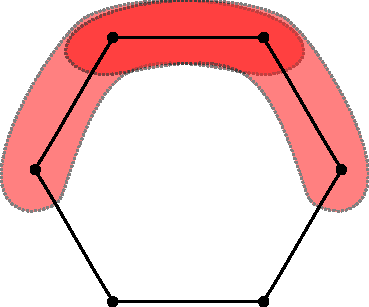
\includegraphics{./images/ring.pdf}
\end{center}
\caption{Overlapping 1-neighbourhoods on a ring}
\end{figure}

\begin{lem} The function $A$ is a valid colouring for the graph $G_{2t+1,n}$.\end{lem}

\begin{pr} Let $\{v,v'\}\in E_{2t+1,n}$ be an edge as above. Assume for the sake of contradiction that $A$ does not produce a valid colouring, i.e. $A(v)=A(v')$. We now construct a ring that is a valid input for the algorithm.

Consider the ring 

\[x_1\rightarrow \ldots \rightarrow x_{t+1} \rightarrow x_{t+2} \rightarrow \ldots \rightarrow x_{2t+1} \rightarrow x_{2t+2} \rightarrow \ldots \rightarrow x_1\] 

%picture ring with vertices x_1... x_t+1 x_t+2 ... x_2t+1,x_2t+2

Since the algorithm produces a valid colouring it colours $x_{t+1}$ and $x_{t+2}$ with different colours. But then the function must be $A(v)\neq A(v')$.
\end{pr}

It follows that $\chi(G_{2t+1,n})\leq 3$. We now show that the chromatic number is actually larger, if $t$ is too small.

\begin{Def} For a graph $\vec G$, the line graph $L(\vec D)$ is  the graph with the same vertex set as $\vec D$ and $(e,e')$ is an edge if e ends where e' starts. 

\begin{figure}[hbt]
\begin{center}
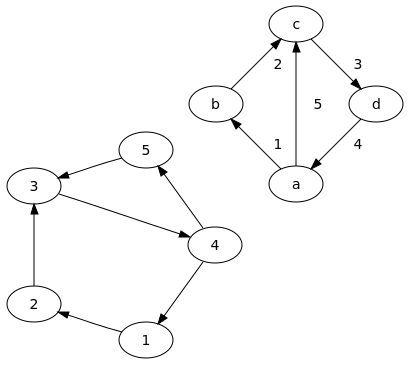
\includegraphics[width=0.8\linewidth]{./images/linegraph_ex}
\end{center}
\caption{A graph and its linegraph}
\end{figure}
\end{Def}

\begin{lem} $\chi(G_{2t+1,n}) \geq \log^{(2t)} n$\end{lem}

\begin{pr} Define a new, directed graph $\vec G_{s,n} = (\vec W_{s,n}, \vec E_{s,n})$ that is build from a subset of the originial graph

\[\vec W_{s,n} = \{(x_1,x_2,\ldots,x_s) | 1\leq x_1\leq \ldots \leq x_s \leq n\}\]
\[\vec E_{s,n} = \{(\underbrace{(x_1,\ldots,x_s)}_{v},\underbrace{(x_2,\ldots,x_{s+1})}_{v'})| v,v'\in \vec W_{s,n} \wedge x_{s+1} > x_s\}\]

Since both the edge and the nodeset of $\vec G$ is a subset of $G$, we immediately have $\chi(\vec G)\leq \chi(G)$. By introducing the new graph we gained the ability to recursively characterize $\vec G_{s,n}$.

\begin{enumerate}
\item $\vec G_{1,n}$ is the complete graph ($i\rightarrow i'$, if $i'>i$). This follows from the definition.
\item $\vec G_{s+1,n} = L(\vec G_{s,n})$

Take $s=3$ as example, see figure \ref{fig:g3_l3}.

\begin{figure}[hbt]
\begin{center}
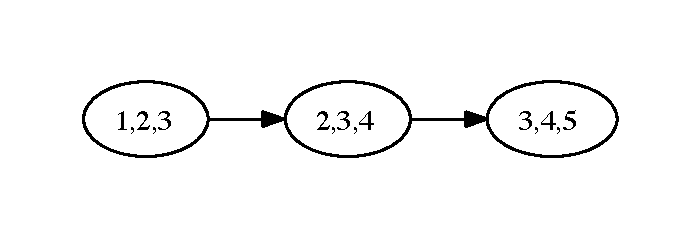
\includegraphics[width=0.58\linewidth]{./images/g3_extr} 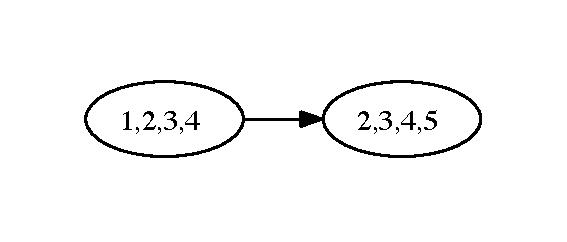
\includegraphics[width=0.4\linewidth]{./images/L(G3)}
\end{center}
\caption{A part of $\vec G_{3,n}$ and the corresponding part of $L(\vec G_{3,n})$}
\label{fig:g3_l3}
\end{figure}

We can identify the edges with elements from $\vec G_4$. And if we don't include an edge in the line graph, we also don't see it in $G_4$.

This also works in the general case: Every time we see an edge in $G_{s,n}$ we map the edge to the union of its endpoints, i.e. a node in $G_{s+1,n}$. If two edges are adjacent s.t. they are a new edge in the line graph, then the union is such that the edge is also in $G_{s+1,n}$
\end{enumerate}
\end{pr}

\begin{lem} $\chi(L(\vec D)) \geq \log \chi(\vec D)$ \end{lem}

\begin{pr} Let $k=\chi(L(\vec D))$ and $\phi$ be a k-colouring. $\phi$ is a colouring of the edges of $\vec D$, since it is a colouring of the line graph.

\begin{center}
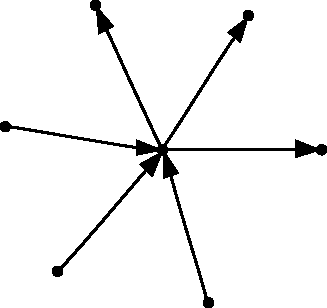
\includegraphics{./images/edge_coloring_line_graph}
\end{center}

For all incoming edges to a, all outgoing edges have a different colour in $\phi$, otherwise it wouldn't be a valid colouring for the line graph.

We construct a colouring $\hat \phi$ of $\vec D$ that uses at most exponentially more colours. 

\[\hat \phi(v) = (b_1,\ldots,x_k)\qquad b_i= \begin{cases} 1 & \exists \text{incoming edge with colour } i\\0 & \text{otherwise}\end{cases}\]

$\hat \phi$ is a valid colouring.

\begin{center}
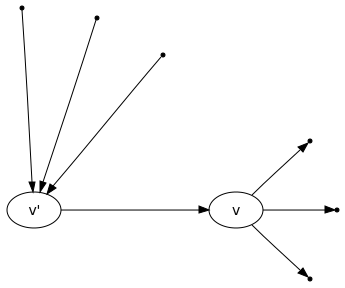
\includegraphics{./images/coloring_from_edges}
\end{center}

Suppose $b_i(v)=1$, then $b_i(v')=0$ otherwise we wouldn't have a valid edge colouring. Since we have $k$ bits available, we can use at most $2^k$ colours in $\hat \phi$.

\end{pr}

\begin{pr}[Theorem \ref{thm:ring_colour_lowerbound}] We need $t=\Omega(\log^* n)$ s.t. $\log^{(2t)} n$ is $\leq 3$.\end{pr}

\paragraph{Remark.}

\begin{itemize} 
\item$G_{s,n}$ doesn't have the nice recursive property. See the example in figure \ref{fig:g_3_counterex}

\begin{figure}[hbt]
\begin{center}
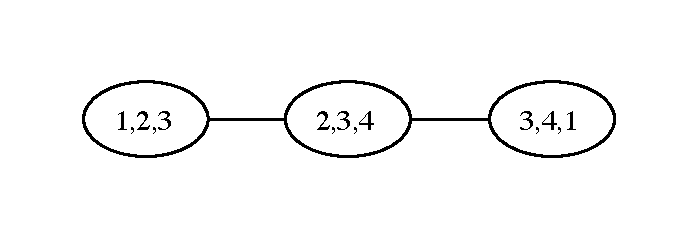
\includegraphics{./images/g_3_counterex}
\end{center}
\caption{The corresponding edge in the line graph $1,2,3,4 \rightarrow 2,3,4,1$ doesn't exist in $G_{4,n}$}
\end{figure}

%1,2,3 -- 2,3,4 -- 3,4,1
%
%a [label ="1,2,3"]
%b [label ="2,3,4"]
%c [label ="3,4,1"]
%
%a -- b -- c
%
%a [label ="1,2,3,4"]
%b [label ="2,3,4,1"]
%a -- b //does not exist
%1,2,3,4 -/- 2,3,4,1
\item The theorem \ref{thm:ring_colour_lowerbound} can be generalised to other graphs too.
\end{itemize}

\section{MIS --- Maximal Independent Set}

\begin{Def} Given an undirected graph $G=(V,E)$ an independent set $U\subseteq V$ is a subset s.t no two vertices in it are connected by an edge:

\[\forall u,v \in U \{u,v\}\not \in E\]

$U$ is \emph{maximal}, if no vertex can be added s.t. this property is preserved. Note the difference to a \emph{maximum} independent set: $U$ is \emph{maximum} if its cardinality is maximal among all independent sets.
\end{Def}

Note that the maximum set anddn a maximal set can be very different 

%picture 
\begin{figure}[hbt]
\begin{center}
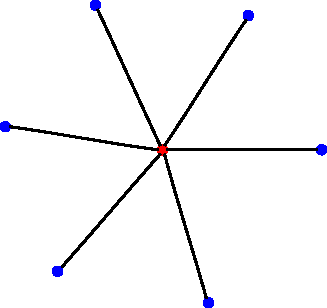
\includegraphics{./images/mis}
\end{center}
\caption{Red node is a maximal independent set, blue are a maximum independent set}
\end{figure}


Finding a maximum independent set is NP-complete, it is even inapproximable by a factor of $\approx \sqrt{n}$ unless P=NP. However maximal independent sets can be computed greedily. We want  to find a distributed algorithm for this problem.

There is a relation between colouring and MIS. Each color class in a coloured graph is an independent set, since there musn't be edges between nodes of the same colour. However it may not be maximal, but we can construct one in a distributed fashion by parallely adding vertices of other colours greedily.

\begin{thm} Given a synchronous distributed algorithm that colours a graph in $R$ rounds with $C$ colours, then we can find a MIS in time $O(R+C)$\qed\end{thm}

\begin{cor} There is a $O(\log^* n)$ algorithm for trees and bounded degree graphs\end{cor}

\subsection{A randomized algorithm}

Here we don't have to assume an initial colouring. Algorithm \ref{alg:fast_mis} runs in phases.

\begin{figure}
\begin{lstlisting}
repeat
	$c$ =  random [0,1] uniformly 
	send $c$ to all neighbour
	
	if $c_v< c_w$ for all $w\in adj(v)$ 
		enter MIS

until $v$ or $w\in adj(v)$ entered
\end{lstlisting}
\caption{Fast-MIS}
\label{alg:fast_mis}
\end{figure}

The algorithm terminates with probability 1, since with probability 1 there is a global smallest random choice, so at least one vertex stops in each round. It also produces a MIS, because as long as a vertex can enter, the algorithm won't stop.


We now want to show that this algorithm takes logarithmically many steps in expectation. We will look at the edges of the graph. We remove edges if they are incident to vertices that stop. We'll show that in expectation half the edges are removed in every round. 

Let $G_i=(V_i,E_i)$ be the graph at the beginning of the $i$th round. Obviously this is a random graph, as it results from a random process. Let $X_i$ be the random variable indicating the number of removed edges in phase $i$.

\begin{lem} \label{lem:at_least_half}$\E(X_i |G_i = G) \geq |E(G)|/2$ \end{lem}

\begin{pr} Define an event
\[E_{v\rightarrow v'} \forall w\in adj(v): c_v<c_w \wedge \forall w\in adj(v') \backslash {v} : c_v < c_w\]
to be the event that the edge ${v,v'}$ is removed because $v$ entered the maximal independent set and $v$ had the smallest random value of all neighbours of $v'$.

\begin{align*}
P(E_{v\rightarrow v'}) &= \frac{1}{| adj(v) \cup adj(v') |}\\
	&\geq \frac{1}{deg(v) + deg(v')}	
\end{align*}

Define a random variable 

\[Y_{v\rightarrow v'} = \begin{cases} \deg(v') & E_{v\rightarrow v'} \text{ occured} \\ 0 & \text{othw.}\end{cases}\]

that counts the edges that are incident to $v'$ and let $Y=\sum_{v,v'} Y_{v\rightarrow v'}$. By linearity of expectation we have

\begin{align*}
\E(Y) &= \sum_{v,v'} \E(Y_{v\rightarrow v'}) + \E(Y_{v'\rightarrow v}) \\
	&\geq \sum_{v,v'} \frac{d(v')}{d(v)+d(v')} + \frac{d(v)}{d(v')+d(v)}\\
	&= |E(G)|
\end{align*}

Let us now consider the relationship between $Y$ and $X_i$. Consider an edge $e={v,v'}$ as in figure \ref{fig:at_least_half} that is removed. $e$ gets counted in $Y$ if $E_{x\rightarrow v'}$ or if $E_{y\rightarrow v}$ happened. So each deleted edge gets counted up to two times. It can not happen that for example $E_{x'->v'}$ happens simultaneously with $E_{x\rightarrow v'}$, because we requested $x$ to be the minimal random value among all neighbours. Hence $X_i \geq Y/2$.

\begin{figure}
\begin{center}
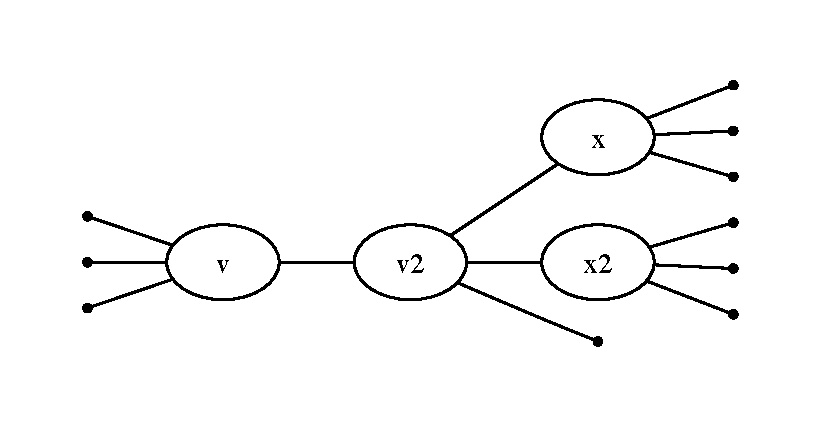
\includegraphics{./images/randomized_matching_delete_edge}
\end{center}
\caption{What edges can be deleted in one round?}
\label{fig:at_least_half}
\end{figure}
\end{pr}

Lemma \ref{lem:at_least_half} alone is not sufficient to prove the logarithmic running time, as the individual stages during the run of the algorithm are not independent\footnote{I think}. We need some more information before we can conclude the bounds on the running time.

\begin{lem} For all $i\geq 1$
\[P(|E_i| \geq 1) \leq |E_1| \cdot 2^{-i+1}\]
\end{lem}

\begin{pr} By Markov's inequality $P(|E_i| \geq 1) \leq \E(|E_i|)$. We want to show that $|E_i|\leq |E_1|\cdot 2^{-i+1}$.

We apply the law of total expectation\footnote{I think that's what it's called} and the previous lemma:

\begin{align*}
\E(|E_i|) &= \sum_{G\subseteq G_1} P(G_{i-1} =G) \cdot \E(|E_i| | G_{i-1}=G)\\
	&=\sum_{G\subseteq G_1}  P(G_{i-1} =G) \cdot \E(|E_{i-1}| -X_{i-1} | G_{i-1}=G)\\
	&=\sum_{G\subseteq G_1}  P(G_{i-1} =G) \cdot (\E(|E_{i-1}| | G_{i-1}=G) - \E( -X_{i-1} | G_{i-1}=G))\\
	&=\sum_{G\subseteq G_1}  P(G_{i-1} =G) \cdot (|E(G)| - \E(X_{i-1} | G_{i-1}=G))\\
	&\stackrel{\text{lem. \ref{lem:at_least_half}}}{=} \sum_{G\subseteq G-1}  P(G_{i-1} =G) \cdot (|E(G)| - \frac{|E(G)|}{2})\\
	&=\frac 12 \sum_{G\subseteq G-1}  P(G_{i-1} =G) \cdot |E(G)|\\
	&=\frac 12 \E(|E_{i-1}|)\\
\end{align*}

By induction we get the bound claimed in the lemma.
\end{pr}

\begin{lem} Let T be the number of rounds until Fast-MIS terminates. Then $\E(T) \leq 2\log n+O(1)$\end{lem}

\begin{pr} We have

\begin{align*}
\E(T) &= \sum_{i\geq 1} i P(T=i) \\
	&= \sum_{i\geq 1} P(T\geq i)\\
	&\leq C + \sum_{i> C} P(T\geq i)\\
\intertext{Note that $P\geq i$ implies $|E_i|\geq 1$, otherwise the algorithm would have stopped.}
	&\leq C+ \sum_{i> C} P(|E_i|\geq 1)\\
	&\leq C+ \sum_{i>C} |E_1|\cdot 2^{-i+1}\\
	&\leq C+ n^2 \cdot \sum_{i>C} 2^{-i}\\
	&\leq C+ n^2 \cdot 2\cdot 2^{-C}\\
\end{align*}

Choose $C$ to be $2\log n$ to get the result.
\end{pr}

\paragraph{Remark.} The algorithm may be fast in expectation, but that doesn't guarantee an acceptable running time with high probability. We would like to have a good running time with probability at least $1-n^{-c}$.

\begin{thm} $P(T> c\log n) = O(n^{2-c})$\end{thm}
\begin{pr} $T>i$ implies $E_i\geq 1$, so $P(T > i) \leq |E_1| \cdot 2^{-c\log n} = n^{2-c}$.\end{pr}

\paragraph{Remark.} \begin{enumerate}
\item We don't need to draw real numbers. It is sufficient to communicate $O(\log n)$ bits (exercise). 
\item It's an open problem to beat $O(\log n)$ randomized rounds. There is no known deterministic algorithm that has logarithmic running time.
\end{enumerate}

\subsection{Applications}

\subsubsection{General Graph Colouring}

We already know how to colour graphs of bounded degree in $O(\log^* n)$. We can use algorithm \ref{alg:fast_mis} to colour general graphs in logarithmic time. We construct an auxiliary graph $G^* = (V^*, E^*)$ out of $G$ by doing the following steps

\begin{enumerate}
\item For every $v\in V$ make $d(v)+1$ clones $C_v = \{v_0,v_1,\ldots v_{d(v)}\}$. $V^*$ is the set of all clones.
\item $C_v$ forms a clique in $G^*$
\item If $\{u,v\} \in E$ then $\{u_i,v_i\} \in E^*$ for $0\leq i \leq \min \{d(u),d(v)\}$, i.e. connect the cliques as in figure \ref{fig:colour_via_matching}

\begin{figure}
\begin{center}
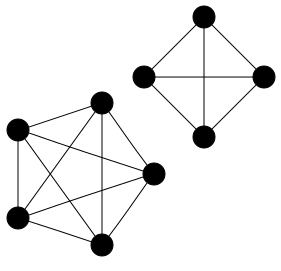
\includegraphics[scale=0.7]{./images/colour_via_matching}
%\begin{verbatim}
%graph G {
%
%	subgraph cluster2 {
%		label = "A"
%		a -- b
%		a -- c
%		a -- d
%		a -- e
%		b -- c
%		b -- d
%		b -- e
%		c -- d
%		c -- e
%		d -- e
%		
%	}
%	
%	subgraph cluster1 {
%	  label = "B"
%		f -- g
%		f -- h
%		f -- i
%		g -- h
%		g -- i
%		h -- i
%	}
%	
%	a -- f
%	b -- g
%	c -- h
%	d -- i
%}
%\end{verbatim}
\end{center}
\caption{Connecting the cliques}
\label{fig:colour_via_matching}
\end{figure}
\end{enumerate}

\begin{figure}[hbt]
\begin{lstlisting}
simulate Fast-Mis($G^*$) //only local information needed
if $v_i\in $ MIS, then
	$c_v=i$ 
\end{lstlisting}
\caption{An algorithm for general graph colouring}
\label{alg:general_colouring}
\end{figure}

\begin{thm} Algorithm \ref{alg:general_colouring} finds a valid colouring with $\leq \Delta+1$ colours in expected time $O(\log n)$.\end{thm}

\begin{pr} Observations:

\begin{enumerate}
\item Since the clones of a node are in a clique, at most one of them can be in the MIS
\item Let $v\in V$ be any vertex and let $w_1,\ldots,w_d$ be its neighbours in $G$

%picture
Since in the clique are $d+1$ vertices, but it only has $d$ edges to neigbouring cliques, one vertex must be free to join the MIS.

\end{enumerate}

So we get a colouring. We have to show that it's valid, i.e. the indices chosen into the MIS are not equal for neighbouring cliques. But this is obvious, since we have $\{u_i,v_i\}$ edges between cliques.

Since copying the nodes only makes the graph polynomially larger, the logarithmic running time is preserved.
\end{pr}
\section{Spanning Trees}
\subsection{Preliminaries}

A spanning tree $T$ of a graph $G$ is a subgraph of $G$ that is a tree and contains all nodes. In a spanning tree any pair of vertices $(u,v)$ is connected by a unique path. Having unique paths in computer networks makes it possible to route messages more efficiently. Obviously some spanning trees are more useful for communication than others, cf figure \ref{fig:not_all_trees_equal}. Graphs/spanning trees with small diameter\footnote{The length of the longest shortest path between any two nodes in the graph} are desirable.

\begin{figure}[hbt]
\begin{center}
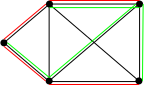
\includegraphics[scale=1.5]{./images/not_all_trees_equal}
\end{center}
\caption{The green tree is more desirable since the diameter is smaller}
\label{fig:not_all_trees_equal}
\end{figure}

Recall that in unweighted graphs the BFS tree is a tree of shortest paths from the root to all other vertices.

\begin{lem} If $T$ is a spanning tree of $G$, the diameter of $T$ is at least as large as the diameter of $G$.\end{lem}

\begin{pr} Obvious, since $T$ is obtained by removing edges from $G$, paths can only get longer.\end{pr}

The gap between the diameter of $G$ and a spanning tree $T$ can be on the order of $n$, cf. figure \ref{fig:diameter_ratio_spanning_tree}. For BFS trees its not so bad though.

\begin{figure}
\begin{center}
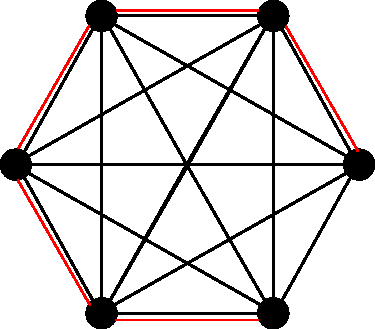
\includegraphics{./images/diameter_ratio_spanning_tree}
\end{center}
\caption{An example for a bad spanning tree}
\label{fig:diameter_ratio_spanning_tree}
\end{figure}

\begin{lem} The diameter of a BFS tree $T$ is at most twice the diameter of $G$\end{lem}
\begin{pr} In any tree $T$ the following holds for the distances:

\[d_T(u,v) \leq d_T(u,r) + d_T(r,v)\]

Since the BFS tree is a tree of shortest paths from the root, we have $d_T(u,r), d_T(r,v) = d_G(u,r), d_G(r,v)$. Since both distances are smaller than the diameter, the bound follows\end{pr} 

\subsection{Broadcasting and Spanning Trees}

Suppose we have a graph $G$ with a node $r\in V$ that wants to broadcast something to all other nodes. Let $D$ be the diameter of $G$ and $R$ be the radius\footnote{The maximal distance of a node to $r$} of $r$. Note $R\leq D\leq 2R$.

\begin{figure}
\begin{lstlisting}
wait for message
forward the message to all other neighbours 
//no loop!
\end{lstlisting}
\caption{Flood: $r$ starts by sending a message, all others perform as in the listing}
\label{alg:flood}
\end{figure}

\begin{thm} Flood informs all vertices. It has time complexity O($D$) and communication complexity\footnote{the number of messages sent} O($m$)
\end{thm}

\begin{pr} The correctness is proved by induction. After $i$ units of time, all vertices at distance $\leq i$ from the root are informed. The vertices at distance $i+1$ have neighbours at distance $i$ that forward them the message.

The communication complexity is also correct, since each node sends $\deg(v)$ many messages. By the handshaking lemma this is $2E$ in total.
\end{pr}

We can extend algorithm \ref{alg:flood} to build a spanning tree by having each vertex set its parent as the node from which it receives the message first. In a synchronous setting it might happen that more than one neighbour sends the message simultaniously; these ties are broken arbitrarily. In any case the decision is transmitted to the parent.

Once the tree is constructed the message complexity for any further broadcasts is reduced to $O(n)$, as messages are only relayed along the tree edges. This is obviously optimal.

But is $T$ a BFS-tree? This depends on the model of computation. In a synchronous setting, where all messages travel at the same speed, we do indeed get a BFS-tree. Not so in an asynchronous setting.

\subsection{BFS-trees in Asynchronous Settings}

There are several approaches to the problem. One solution works in phases: in phase $p$ all nodes at distance $p$ are included in the tree (exactly as in the synchronous setting). The phases are synchronised by the root. At the end of the phase all nodes send a message to the root and the root sends the "ok" back to start a new phase. The overhead for the synchronization is $2p$ after phase $p$. Since $p\leq D$ (actually $\leq R$) we get a time complexity of $O(D^2)$ in total. The message complexity is O($m+nD$).

This synchronization method is useful in other settings too.
\section{Minimum Spanning Trees -- The GHS Algorithm}
\subsection{Overview}

We want to find a minimum spanning tree\footnote{The sum of the edge weights in T is minimal over all spanning trees} in a weighted graph in an asynchronous setting. 

\begin{Def}[Fragment] A fragment of a tree T is a connected subgraph of T. \end{Def}

The algorithm will work similarly to Kruskal's algorithm in that we start with single vertices and build lightest fragments, merging them eventually to obtain a spanning tree. The correctness of this idea relies of the following lemma:

\begin{lem} Let $F$ be a fragment of an MST and let $e$ be an outgoing edge\footnote{an edge that connects a node of $F$ with a node $v\in V\backslash F$} of minimum weight. Then $F\cup \{e\}$ is also a fragment of an MST (possibly a different one).\end{lem}

\begin{pr} Let $T$ be an MST containing $F$ and suppose $e$ is not in $T$. Add $e$ to $T$; it must close a cycle. The cycle has some other edge $e'$ that is also an outgoing edge of $F$. Since $e$ has minimal weight over all outgoing edges, removing $e'$ and adding $e$ to $T$ can only yield a tree of smaller or equal weight.\end{pr}

To make things easier we will assume that all weights are distinct.

\begin{lem} If all edge weights are distinct, the MST is unique \end{lem}
\begin{pr} Suppose for the sake of contradiction that $T,T'$ are different MSTs. Let $e$ be the lightest edge of $T$ or $T'$ that is not contained in both trees. W.l.o.g $e\in T$. 

Let $H$ be $T'\cup \{e\}$. Again the additional edge closes a cycle in $T'$. There must be some edge $e'$ on the cycle that isn't in $T$. Since $e$ was the lightest such edge and all weights are different, $w(e')\gneq w(e)$. Hence removing $e'$ would make $T'$ lighter.\end{pr}

In an asynchronous setting we can't simply sort the edges by weight and add them one after the other unless they close cycles. Instead we will proceed as follows:

Fragments will find their minimal outgoing edge. We also assign levels to fragments (initially 0). Let $L,L'$ be the levels of neighbouring $F$ and $F'$. Two fragments merge if 

\begin{enumerate}
\item $L<L'$ with new level $L'$
\item $L=L'$ and the minimum outgoing edge of $F$ and $F'$ coincide (the new level is $L+1$)
\end{enumerate}

otherwise $F$ waits. The termination is guaranteed as after a while only one fragment is left. Until that happens there is always one globally lightest edge between two fragments that will get the fragments to merge.

\subsection{The Algorithm}

Of course coordinating the fragments is quite complicated. The vertices are in one of three states

\begin{description}
\item[Sleeping] The initial state
\item[Find] this vertex is currently participating in finding the minimum weight outgoing edge
\item[Found] all other times
\end{description}

%Sleeping -> Found [label = "Connect(0)"]
%Found -> clusterFind [label = "Init(L,ID)"]
%subgraph clusterFind {
%	one [label = "Find min outg. edge"]
%	one -> two
%	two [
%}

The edges also have states

\begin{description}
\item[Basic] the default state
\item[Branch] this edge is in the MST
\item[Rejected] the edge that is not in the MST (it connects two nodes in a fragment, but it's not a Branch)
\end{description}

When a vertex is awakened it chooses the minimum-weight incident edge and sends a {\scshape Connect(0)} and switches to state Found. 

Suppose that a fragment of level $L$ has just been formed out of two level $L-1$ fragments via the outgoing edge $e$. $e$ is now the \emph{root} of the new fragment and $w(e)$ is the ID of the new fragment. $u,v$ must now broadcast this information to the other nodes by sending {\scshape Init(L,ID)}. All receiving vertices go to the state Find and start searching for an outgoing edge of minimal weight.

If a fragment with higher ID is created it may be that other fragments are waiting to connect. The {\scshape Init} message is also forwarded to neighbours with outstanding {\scshape Connect} requests. They then join the new fragment.

In the Find state vertices find their lightest outgoing edge and cooperate with the other vertices to find the globally lightest. During the first stage {\scshape Test(ID)} messages are sent over Basic edges. If the receiver has the same ID, the edge is Rejected (these edges close cycles). Otherwise the receiving node checks whether its level is greater or equal that of the sender, in which case the edge is Accepted. If however the level is smaller, it waits until the above conditions become true.

Afterwards, in the second state all leaves {\scshape Report} their state to their neigbours. All internal nodes wait until they have gathered the information from the children and then report themselves. When the report arrives at $u$ and $v$ they can decide which is the smallest outgoing edge in the whole fragment and broadcast ({\scshape Trace\_Back}) that information to the other nodes. After the broadcast completes the vertices switch to Found.

It is also possible that $v$ sends {\scshape Connect} to a vertex $w$ in a fragment with higher ID. Since the fragments will merge immediately an {\scshape Init(L,ID)} message is send back to $v$. There are two cases: Either $w$ has already reported the minimum weight outgoing edge to the parent or it hasn't. In the latter case the fragment of $v$ participates in finding the minimum weight outgoing edge. If $w$ however has already sent {\scshape Report}, it means that some other edge $e'$ besides $(v,w)$ is the minimum weight outgoing edge of $w$ (otherwise a {\scshape Test} would have been sent to $v$). But in this case the outgoing edges of $v$'s fragment all must have greater weight than those of $w$'s fragment.

\begin{lem} A fragment at level $l$ contains $\geq 2^l$ vertices.\end{lem}
\begin{pr} The level only increases if two same size fragments are merged, the rest follows by induction.\end{pr}

So the highest level is at most logarithmic in the number of vertices.

\begin{lem} The message complexity of the algorithm is O($|E|+|V|\log |V|$)\end{lem}
\begin{pr} We count the different messages separately:
\begin{itemize}
\item {\scshape Test} At most one in each direction on each edge.
\item {\scshape Accept/Reject} Same as {\scshape Test}
\item {\scshape Init} once per level all nodes get informet, $\leq |V|\log |V|$
\item {\scshape Connect} at most two per edge
\item {\scshape Report} same as {\scshape Init}
\item {\scshape Trace\_Back} same as {\scshape Init}
\end{itemize}
\end{pr}
\section{Routing and Small Worlds}

See \href{http://en.wikipedia.org/wiki/Small_world_experiment}{Wikipedia:Small world experiment} for the general setting.

\subsection{Model and Decentralized Algorithms}

The first observation is that real networks, e.g. social networks, are rich in local connections: we know many people in our university, but few people in neigbouring cities. The model should reflect that. We consider a superposition of two graphs.

Let $G_n(l,f,\alpha)$ be the graph we will consider. The vertex set are points on a $\sqrt{n}\times \sqrt{n}$ grid. Distance $d(u,v)$ between vertices is computed by Manhatten distance. We have two kinds of edges:

\begin{itemize}
\item \emph{Local contacts}: Each vertex is connected to all vertices at distance $\leq l$
\item \emph{Far contacts}: Every vertex has $f$ far contacts, that are randomly chosen. The probability to choose an edge $(u,v)$ is proportional to $d(u,v)$
\[P(\text{$u$ chooses $v$}) = \frac{d(u,v)^{-\alpha}}{\sum_{w\neq u} d(u,w)^{-\alpha}}\]
\end{itemize}

In the pure grid graph with only local contacts the diameter is very high, on the order of $\sqrt n$. Adding random neighbours changes this. The factor $\alpha$ regulates how important the distance is for the probability to choose neighbours. At $\alpha=0$ we have a uniform distribution.

We want to send messages along "short" paths in this graph. We assume that the algorithm knows the local connections of all vertices and the coordinates of the target node $t$. Under certain circumstances we will also assume that we know all the far edges of the previous hops. Let's call such algorithms \emph{decentralised}.

\begin{thm}\label{thm:small_world_graphs} Let $l,f\geq 1$ and let $0\leq \alpha \leq 2$. There is a constant $c=c(l,f,a) > 0$ such that if D denotes the diameter of $G_n(l,f,\alpha)$ then $P(D<c\log n) \geq 1-o(1)$
\end{thm}

Note that if $\alpha \geq 2$ the statement becomes false (the diameter becomes $n^\epsilon$ with $\epsilon > 0$). The next statement concerns finding such paths.

\begin{thm}\label{thm:finding_short_paths} \mbox{}\begin{enumerate}
\item Let $l=f=1$, $\alpha =2$. Then there is a decentralised algorithm $A$ with expected delivery time $O(\log^2n)$
\item Let $l,f\geq 1$, $0 \leq \alpha \lneq 2$. Then there is a $c=c(l,f,\alpha)>0$ such that the expected delivery time of any decentralized algorithm is at least $c n^{\frac{2-\alpha}{3}}$.
\end{enumerate}
\end{thm}

Recall: If $X = \sum_{i=1}^n X_i$
\begin{align*}
Var(X) &= \E\left(\left(\sum X_i\right)^2\right) - \E\left(\sum X_i\right)^2\\
	&= \sum_{1\leq i, j\leq n} (\E(X_iX_j) - \E(X_i)\E(X_j))
\end{align*}

also useful: \href{http://en.wikipedia.org/wiki/Chebyshev\%27s_inequality}{Wikipedia:Chebyshev's inequality}. Further:

\begin{lem} Let $0\leq x \leq 1$. Then
\begin{enumerate}
\item $1-x\leq e^{-x}$
\item $e^{-x} \leq 1-x+\frac{x^2}{2}$
\end{enumerate}
\end{lem}
\begin{pr} Consider the series expansion:
\[e^{-x} = \sum_{i\geq 0} \frac{(-x)^i}{i!} = 1-x+\frac{x^2}{2} - \ldots\]
1. holds because 
\[\sum_{i\geq 1} \frac{x^{2i}}{(2i)!} - \frac{x^{2i+1}}{(2i+1)!} \geq 0\]
and 2. holds because
\[\sum_{i\geq 1} \frac{x^{2i-1}}{(2i-1)!} - \frac{x^{2i}}{(2i)!} \geq 0\]
\end{pr}

\begin{pr}[Theorem \ref{thm:small_world_graphs}] We will assume $\alpha=0$ and $n$ "large enough" to make things easier. Under these assumptions $\forall u: \sum_{v\neq u} d(u,v)^{-\alpha} = n-1$. 

For $S\subset V$ let 
\[X(S) = \bigcup_{v\in S} \tilde N(v) \backslash S\]

where $\tilde N(v)$ is one far-away neighbour $f_v$ of $v$ and $f_v$'s right neighbour. Let $C_0$ be the upper left subgrid of sidelength $\log n$ and let

\[C_{i+1} = X(C_{i-1})\]

We will show that 

\begin{enumerate}
\item with probability $1-o(1/\log n)$ we have $|C_i| \geq 1.5 |C_{i-1}|$, as long as $|C_i| \leq 8 \frac{n}{\log n}$. So after few iterations we see many vertices. 
\item Let $i^*$ be the smallest $i$ s.t. $|C_i| \geq 8\frac{n}{\log n}$. We then proceed to show that every vertex that is not in $C_{i^*}$ can be reachen in O($\log n$) steps.
\end{enumerate}

From these facts follows the theorem, as we can go from any vertex to a vertex in $C_{i^*}$ in O($\log n$) steps, proceed to $C_0$ and take the direct route there ($C_0$ has small diameter).

Let $v\not \in C_{i-1}$. Define a random variable $X_v$ that is $1$ if $v\in C_i$.

\[X_v = \begin{cases} 1& \exists v'\in C_{i-1}: v\in \tilde N(v')\\ 0& \text{otherwise}\end{cases}\]

Clearly the sum of these variables is exactly $|C_i|$. We use Chebishev to bound the size of $C_i$ (so we first compute the variance). Let $|C_i| = S$

Since $X_v$ is an indicator variable we have 

\[\E(X_v) = 1-P(X_v=0)\]
	
$X_v$ is 1 if either $v$ is a far contact of some node, or $v$'s left neighbour, $u$, is such a contact. The probability that one vertex selects $v$ or $u$ is $2/(n-1)$. Since the choices are independent:

\[\E(X_v) = 1-\left(1-\frac{2}{n-1}\right)^S\]

Of course if $v$ is on the left edge of the grid we get $1/(n-1)$, but we'll ignore that for now. For calculating the variances we need $\E(X_uX_v)$ too. We have

\[\E(X_vX_u) = 1-P(X_u=0) - P(X_w=0) + P(X_u=X_v=0)\]

by inclusion-exclusion. The interesting part is $P(X_u=X_v=0)$. There are several cases: If $u$ and $v$ aren't left neighbours of each other and don't lie on the border we mustn't choose one of $4$ nodes. If they lie next to each other there are $3$ forbidden vertices.

\[\E(X_vX_u) = 1-2\left(1-\frac{2}{n-1}\right)^S+\left(1-\frac{\xi}{n-1}\right)^S \quad \xi = \begin{cases}4 &\text{not neighbours}\\ 3 &\text{right neighbours}\end{cases}\]

With these two expectations we can compute the variance. The following formula also considers the edge cases:

\begin{align*}
\E(C_i) &\geq (n-|C_{i-1}| -\sqrt n) \cdot \left(1-\left(1-\frac{2}{n-1}\right)^S\right) \\
 &\geq \left(n- 8\frac{n}{\log n} - \sqrt{n}\right) \cdot \left(1-e^{-\frac{2s}{n-1}}\right)\\
 &\geq \left(n- 9\frac{n}{\log n}\right) \cdot \left(1-e^{-\frac{2s}{n-1}}\right)\\
 &\geq \left(1- 9\frac{n}{\log n}\right)n \cdot \left(1-\left(1-\frac{2s}{n-1}+\frac 12 \left(\frac{2s}{n-1}\right)^2\right)\right)\\
 &\geq \left(1- 9\frac{n}{\log n}\right)\left(2S\left(1+\frac{1}{n-1}-(1+o(1))\frac{2s^2}{n}\right)\right)\\
Since \intertext{$S \in o(n)$}\\
 &\geq (1- o(1))2S\\
\end{align*}
\end{pr}
Now we proceed to calculate the variance:

\begin{align*}
\var(|C_i|) &= \sum_{u,v} \E(X_uX_v) - \E(X_u) \E(X_v)\\
\end{align*}

There are two cases for the summands:

\begin{itemize}
\item $u=v$. We get

\[\var(|C_i|) \leq \E(X_uX_v) = \E(X_u^2) = \E(X_u)\]

The total contribution of these summands is $\leq \E(|C_i|)$

\item $u$ is a left neighbour of $v$. We get

\begin{align*}
\E(X_uX_v) -E(X_u) \E(X_v) &= 1-2(1-\frac{2}{n-1})^S  (1-\frac{3}{n-1})^S -(1-(1-\frac{2}{n-1})^S)^2\\
	&=1-2(1-\frac{2}{n-1})^S+(1-\frac{3}{n-1})^S -(1-2(1-\frac{2}{n-1})^S+(1-\frac{2}{n-1})^{2S})\\
	&=(1-\frac{3}{n-1})^S -(1-\frac{2}{n-1})^{2S}\\
\intertext{As $(1-x)^n\geq 1-nx$}
	&\leq 1 -(1-\frac{4S}{n-1})\\
	&=\frac{4s}{n-1}
\end{align*}
	
There are less than $2n$ such pairs, so we get a total contribution of $\leq \frac{4s}{n-1}2n \leq 9S$

\item $u$ and $v$ are somewhere distributed on the grid. 

\begin{align*}
\E(X_uX_v)-\E(X_u)\E(X_v) &= 1-2(1-\frac{2}{n-1})^S+(1-\frac{4}{n-1})^S-(1-2(1-\frac{2}{n-1})^S +(1-\frac{2}{n-1})^{2S})\\
&= (1-\frac{4}{n-1})^S - (1-Sfrac{2}{n-1})^{2s}\\
&= (1-\frac{4}{n-1})^S-(1-\frac{4}{n-1}+\frac{4}{(n-1)^2})^S\\
\end{align*}

Hence the total contribution is at most $\leq 0$.
\end{itemize}

Combining all the cases we get 

\begin{align*}
\var(|C_i|) &\leq \E(|C_i|) +9S + 0 \\
	&\leq 2s+9S\leq 11S
\end{align*}

By applying Chebychev's inequality we can bound the probability that the $C_i$ don't grow fast enough:

\[P(|C_i| \leq \frac 32 |C_{i-1}|) = P(||C_i| - \E(|C_i|) | \geq \frac 13 |C_i|) \leq \frac{99}{S} = O(\log ^{-2} n)\]

The last equality holds because we start with $S=\log ^2n$. 

This completes the first part of the proof. We have shown that the $C_i$ grow in every step with high probability and hence we reach $C_{i^*}$ in just a logarithmic number of steps. We now want to show that we can reach all nodes from $C_{i^*}$ with only a few additional steps.

We take a $\log n$ sidelength box around a vertex $v$ and show that there is an edge from that box to $C_{i^*}$. Let $Y_v$ be an indicator random variable that is 1 if no vertex in $C_{i^*}$ sends a vertex to the box of $v$. Let $Y=\sum_v Y_v$. We want $Y$ to be $0$ (i.e. all boxes have such an edge) with high probability.

\begin{align*}
P(Y>0) &\leq \E(Y) \\
	&= \sum_v \E(Y_v)\\
	&= \sum_v (1-\frac{\log^2n}{n-1})^{|C_{i^*}|}\\
	&\leq n (e^{-\log^2n/(n-1)\cdot 8\cdot \frac{n}{\log n}})\\
	&\leq n \cdot \exp(-8\log n \cdot \frac{n}{n-1})\\
	&=\exp (\log n - 8(1+o(1))\log n)\\
	&=\exp (-7(1+o(1)) \log n)
	&=o(1)
\end{align*}

This completes the proof for the diameter.
\end{pr}

\begin{pr}[Theorem \ref{thm:finding_short_paths}] For this proof we assume $\alpha=2,l=f=1$. Let $A$ be the current message holder. $A$ passes the message on to that neighbour that is closest to the target (by Manhattan distance). We want to show that the expected travel time of the message is $O(\log^2n)$.

Recall that 

\[P((u,v)\in E_{\text{far}}) = \frac{d(u,v)^{-2}}{\sum_{w\neq u}d(u,w)^{-2}}\]

Let's try to estimate $\sum_{w\neq u}d(u,w)^{-2}$. Let $N_d(u) = |\{w|d(u,w)=d\}|$. Observe:

\begin{align*}
\sum_{w\neq u}d(u,w)^{-2} &= \sum_{d=1}^{\sqrt n} d^2\cdot N_d(u)\\
\intertext{Note: $d\leq |N_d(u)|\leq 4d$ (draw a picture). The lower bound holds for $d\leq (\sqrt n) /2$}
	&\leq \sum_{d=1}^{2\sqrt n} 4 d^{-1}\\
	&\leq 4 \ln(2\sqrt{n})
\end{align*}

We say that $A$ is in phase $J$ if the current distance to $t$ is $2^{j-1} < t \leq 2^j$. Initially $j$ is at most $\log (2\sqrt n)$. It is clear that we have only logarithmically many phases with this definition. We need to bound the time we stay in one phase.

Note: In every step the distance to the target decreases, as each node sends the message to the neighbour that is closest to the target. Hence a vertex is has the message at most once. In particular we haven't seen the far-edge of the current vertex before. We can thus consider it random in every step (the algorithm doesn't change if we generate the far connection as we first reach the vertex).

Suppose $A$ is in phase $j$ at vertex $v$. Let $B_j$ be the number of vertices at distance $\leq 2^{j-1}$ from $t$. 

\[B_j = \sum_{d=1}^{2^{j-1}} N_d(t)\geq \sum_{d=1}^{2^{j-2}} N_d(t)\]

As $2^{j-2} \leq 2^{\log(2\sqrt{n})-2} = \sqrt{n}/2$ and we bounded $d$ we can bound $B_j$

\[B_j \geq \left( {2^{j-2}+1} \atop 2 \right) \geq 2^{2j-5}\]

We can proceed to bound the probability that the algorithm ends in the next step.

\begin{align*}
P(\text{phase ends}) &= \sum_{u\in B_j} \frac{d(v,u)^{-2}}{\sum_{w\neq v} d(v,w)^{-2}}\\
\intertext{Go to $t$ then go to $u$}
&\geq \sum_{u\in B_j} \frac{(2^j+2^{j-1})^{-2}}{4\ln \sqrt{n}}\\
&\geq B_j \cdot \frac{(2^{j+1})^{-2}}{4\ln n}\\
&\geq 2^{2j-5} \cdot \frac{2^{-2j-2}}{4\ln n}\\
&=\frac{2^{-5}}{\ln n}
\end{align*}

So in expectation we need the inverse of that probability many steps until we are done with a phase (formally: define a geometric random variable, find its expectation).

It follows that we need O($\log^2n$) many steps, as there are logarithmically many phases.

We now show the second part of the theorem. Let $0\leq \alpha < 2$ and $l,f\geq 1$. We show there are parameters such that any algorithm has a bad running time.

To show this we make the algorithm slightly stronger. In step $i$ let $S_i$ be the set of vertices that have touched the message. The algorithm can send the message to any neighbour of a vertex in $S_i$. In other words: backtracking is free.

As in the previous case we estimate the probability that $u$ chooses $v$ as a far neighbour.

\[P((u,v)\in E_{\text{far}}) = \frac{d(u,v)^{-\alpha}}{\sum_{w\neq u}d(u,w)^{-\alpha}}\]

We do the same trick as before and split the sum up according to the distance of the nodes.

\begin{align*}
\sum_{w\neq u} d(u,v)^{-\alpha} &\geq \sum_{d=1}^{\sqrt{n}/2} N_d(u)d^{-\alpha}\\
	&\geq \sum_{d=1}^{\sqrt n/2} d^{-\alpha +1}\\
	&\geq \int_1^{\sqrt{n}/2} x^{-\alpha+1}\ dx\\
	&=\left. \frac{x^{-\alpha +2}}{2-\alpha}\right|_1^{\sqrt{n}/2}\\
	&=\frac{1}{2-\alpha} ((\frac{\sqrt n}{2})^{-\alpha +2} -1)\\
	&\geq n^{(2-\alpha)/2} \cdot \frac{1}{2-\alpha} \cdot 2^{\alpha-3}
\end{align*}

So instead of something logarithmic, we got some polynomial. We now show that this happens with high probability.

Take the two vertices $(u,v)$ of the grid s.t. the distance between them is maximal (e.g. the edges of the grid). Let $\delta = \frac{2-\alpha}{6}$ and let $U=\{u|d(u,t) \leq ln^\delta\}$. For the size of $U$ we get $|U| \leq l^2n^{2\delta}$. Let $E_n$ be the event that within $\lambda n^\delta$ steps the message will reach a node that has a for contact in $U$. Let $\lambda = (2^{7-\alpha} \cdot f \cdot l^2)^{-1}$. 

\[E:= \bigcup _{i=1}^{\lambda n\delta} E_i\]

We will show that the probability of the event $E$ ist small. $c_\alpha = \frac{2^{\alpha-3}}{2-\alpha}$

\begin{align*}
P(E_i) &\leq |U| \cdot 2fc_\alpha^{-1} \cdot n^{-\frac{2-\alpha}{2}}\\
	&\leq 2f\cdot c_\alpha^{-1} \cdot l^2 \cdot n^{\frac{2-\alpha}{3} -\frac{2-\alpha}{2}}\\
	&=2f\cdot c_\alpha ^{-1} l^2 \cdot n^{-\delta}
\end{align*}

We can now apply a union bound to get $P(E)$

\begin{align*}
P(E) &\leq\sum_{i=1}^{\lambda n\delta} P(E_i)\\
	&\leq  \lambda n^\delta \cdot 2f\cdot \alpha^{-1} \cdot l^2 n^{-\delta}\\
	&= \frac{1}{2^{7-\alpha} fl^2} \cdot 2f\cdot \frac{2-\alpha}{2^{\alpha-3}} \cdot l^2\\
	&=(2-\alpha)\cdot 2^{-3}\\
	&\leq \frac{1}{4}
\end{align*}

Hence after $\lambda n^\delta$ steps we haven't reached a node with a far contact into $U$ with probability at least $3/4$. And by the definition of $U$ we don't progress fast within $U$ either.\footnote{Why exactly?}.
\end{pr}



\subsection{Greedy Embeddings}

We want to embed the graph in a space such that we can successfully find a path between two nodes just by looking at the neighbours and the knowledge about the coordinates. An embedding $f$ is greedy if for any $s\neq t\in V$ then there is a $v\in N(s)$ such that the distance decreases:

\[d(f(v),f(t)) < d(f(s),f(t))\]

In a greedy embedding any $t\in V$ has an edge to $v$ that is closest in the embedding (otherwise $v$ can't be reached greedily).

For example hamiltonian graphs have a greedy embedding on the euclidian plane (draw them as a line). However not all graphs have such an embedding on the plane.

\begin{lem} $K_{k,5k+1}$, $V=A\dot \cup B$ has no greedy embedding in the euclidian plane. 
\end{lem}

\begin{pr} Assume for the sake of contradiction that $f:V\rightarrow \R$ is a greedy embedding.Let $c(v)$ be the closest vertex in A in $f$. There is a vertex $a\in A$ which is the closest neighbour for $b_1,b_2,\ldots b_6\in B$. The circle around $b_{i+1}$ with radius $d(a,b_{i+1})$ must be empty since it can't contain vertices from $A$ by choice of $a$ and it mustn't contain vertices from $B$ (otherwise there would be edges within $B$). 

% pic star

There must be an angle that is less or equal to the average $\leq \pi/3$. Let $\phi_a\leq \pi/3$ be the angle between $b_i$ and $b_{i+1}$. Consider the triangle $a,b_i,b_{i+1}$. Since the anglesum in triangles is $\pi$ there must also be an angle, wlog the largest of those is $\phi_i$, that is $\geq \pi/3$. But then the distance between $b_i$ and $b_{i+1}$ is defined by the law of sines:

\[\sin \phi_a / d(b_i,b_{i+1}) = \sin \phi_i / d(a,b_{i+1})\]

Since $\phi_a \leq \pi/3 \Rightarrow \sin \phi_a \leq \sqrt{3}/2$. We need $\phi_i\leq 2\pi/3$ and we get

\[\frac{\sqrt{3}}2 \cdot 1\frac{1}{d(b_i,b_{i+1})} \geq \frac{\sin \phi_a}{d(b_i,b_{i+1})} = \frac{\sin \phi_i}{d(a,b_{i+1})} \geq \frac{\sqrt 3}{2} \cdot \frac{1}{d(a,b_{i+1})}\]

And hence $d(a,b_{i+1})\geq d(b_i,b_{i+1})$
\end{pr}

\begin{thm} Every 3-connected planar graph has a greedy embedding. \qed\end{thm}

The theorem is as good as it can be, since we know $K_{2,11}$ (2-connected) and $K_{3,16}$ (3-conn, not planar) have no embedding.

This is however not useful, since the networks we're considering don't have that property.

\subsection{Greedy routing in normed spaces}

Instead of two dimensions we generalize to $f:V\rightarrow \R^n$ and use a different difference metrik. A norm needs to have these properties

\begin{enumerate}
\item $\norm{0} = 0$, $v\neq 0 \Rightarrow \norm{v} >0$
\item $\norm{\alpha v}= |\alpha | \cdot \norm{v}$
\item $\norm{x+y} \leq \norm x +\norm y$
\end{enumerate}

With the norm it is easy to define the distance as the length of the vector between two points.

\begin{lem} Let $(\R^n, \norm{\cdot})$ be a normed space. If it admits a greedy embedding of any graph with $N$ vertices then

\[n \geq \log_3(N-1)\]
\end{lem}

\begin{pr} Consider a star with a central vertex $u$ and $N-1$ vertices around it. Let $f$ be a greedy embedding that maps $u$ to $0$. Let $x_i=f(u_i)$, $l_i=\norm{x_i}$ and $w_i = x_i/l_i$.

Claim: $\norm{w_i-w_j} \geq 1$ if $i\neq j$. Assume otherwise. Consider $d(x_i,x_j)=\norm{x_i,x_j}$.

\begin{align*}
d(x_i,x_j)&=\norm{x_i,x_j} \\
	&=\norm{l_iw_i - l_jw_j}\\
	&=\norm{l_i(w_i-w_j) -(l_j-l_i)w_j}\\
  &\leq l_i \norm{w_i-w_j} + |l_j-l_i|\cdot \norm{w_j} && (l_i\leq l_j)\\
  &< l_i + |l_j-l_i|\\
  &=l_j = \norm{x_j}\\
  &=d(f(u_j),0)
\end{align*}

So the distance between $u_i$ and $u_j$ is strictly smaller than the distance between $u_j$ and the origin, a contradiction.

Hence balls of radius $1/2$ around each $u_i$ is empty and the ball of radius $3/2$ around $u$ contains $N-1$ smaller balls.

\[\Vol(B_{3/2}) \geq (N_1)\Vol(B_{1/2})\]

In normed spaces $\Vol(B_r) = r^n \Vol(B_1)$. We get

\[\frac 32 \Vol(B_1) \geq (N-1)(\frac 12^n \cdot \Vol(B_1)\]

And thus $3^n\geq N-1$
\end{pr}
\end{document}
